\documentclass{documentation}
\usepackage{tikz}
\usetikzlibrary{shapes.geometric, arrows}
\tikzstyle{role} = [rectangle, rounded corners, minimum width=3cm, minimum height=1cm,text centered, draw=black]

\title{Opis systemu ASSASSIN}
\author{Tomasz Chady}

\renewcommand{\figurename}{Schemat}

\begin{document}

\maketitle

\section{Wprowadzenie}

ASSASSIN to system do przechowywania i udostępniania wyników badań pacjentom i personelowi medycznemu.
System jest przeznaczony dla szpitali, klinik i laboratoriów.
Głównym celem systemu jest zapewnienie bezpiecznego dostępu do wyników badań.
System jest dostępny poprzez aplikację mobilną oraz stronę internetową.
Dzięki zaimplementowaniu standardowych informatycznych rozwiązań system jest o wiele bezpieczniejszy i zapewnia większy poziom prywatności niż tradycyjne rozwiązania.

\section{Zakres systemu}

System umożliwia przechowywanie wyników badań pacjentów.
Wyniki badań są dostępne dla personelu medycznego oraz pacjentów.
Personel medyczny może dodawać wyniki badań do systemu.
Pacjenci mogą przeglądać wyniki swoich badań zdalnie przez internet.
Wyniki badań są dostępne poprzez aplikację mobilną oraz stronę internetową i są dostępne tylko dla uprawnionych osób.
Dodatkowo system umożliwia odebranie wyników badań fizycznie w placówce medycznej.
Ogólny schemat systemu jest przedstawiony na schemacie \ref{fig:system}.

\begin{figure}[h!]
    \centering
    \includegraphics[width=0.8\textwidth]{Level_1_C4_Model.png}
    \caption{Schemat systemu ASSASSIN\label{fig:system}}
\end{figure}

\section{Role użytkowników}

System posiada trzy role użytkowników: pacjent, personel medyczny oraz administrator.
Każda rola definiuje co użytkownik może robić w systemie.
Poniżej przedstawiono szczegółowy opis każdej z ról, a na schemacie \ref{fig:roles} przedstawiono graficznie relacje między rolami.

\begin{figure}[h!]
    \centering
    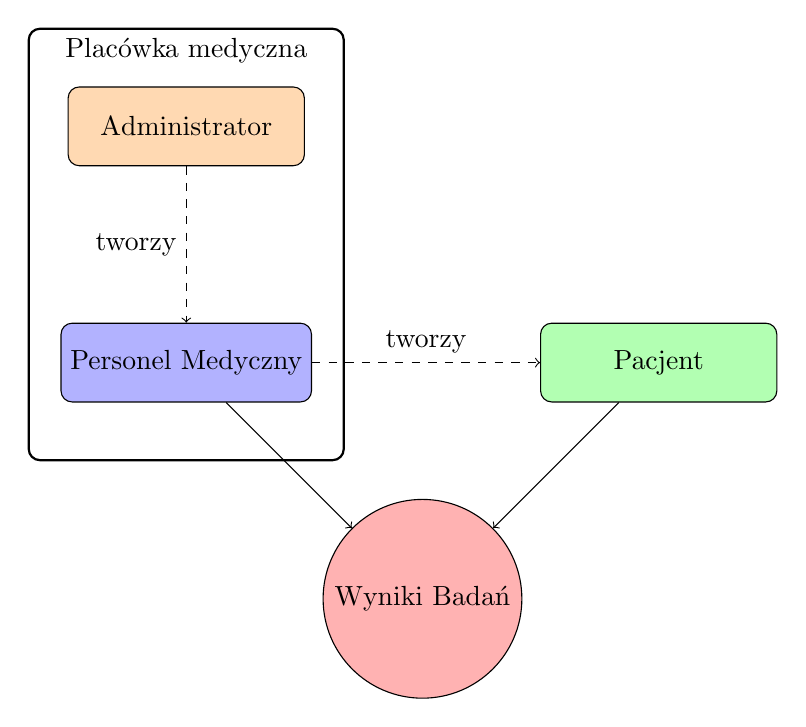
\begin{tikzpicture}[node distance=3cm]
        \node[role, fill=orange!30] (admin) {Administrator};
        \node[role, fill=blue!30, below of=admin, xshift=0] (med) {Personel Medyczny};
        \node[role, fill=green!30, below of=admin, xshift=6cm] (patient) {Pacjent};
        \node[circle, draw=black, fill=red!30, below of=med, xshift=3cm] (data) {Wyniki Badań};
        \node (rect) at (admin) [draw,thick,minimum width=4cm,minimum height=5cm, rounded corners, yshift=-1.5cm, text depth = 5 cm] {Placówka medyczna};

        \draw [dashed, ->] (admin) -- node[anchor=east]{tworzy} (med);
        \draw [dashed, ->] (med) -- node[anchor=south]{tworzy} (patient);
        \draw [->] (patient) -- (data);
        \draw [->] (med) -- (data);
    \end{tikzpicture}
    \caption{Schemat ról w systemie ASSASSIN\label{fig:roles}}
\end{figure}

\subsection{Pacjent}

Konto pacjenta jest tworzone przez personel medyczny podczas pierwszego kontaktu z pacjentem.
Pacjent identyfikowany jest poprzez anonimowy login, hasło oraz aplikację 2FA.
W ten sposób minimalizowane jest ryzyko wycieku danych osobowych pacjenta poprzez błąd użytkownika.
Pacjent może przeglądać wyniki swoich badań oraz odbierać wyniki badań fizycznie w placówce medycznej.
Ewentualne przejęcie konta pacjenta przez osobę trzecią nie powinno spowodować katastrofalnego wycieku danych osobowych, albowiem system minimalizuje ilość przechowywanych danych.
Dobrze to wpływa na koszty utrzymania systemu oraz na bezpieczeństwo użytkowników.

\subsection{Personel Medyczny}

Konto personelu medycznego jest tworzone przez administratora.
Jest ono powiązane z konkretną placówką medyczną oraz konkretnym nazwiskiem.
Autoryzacja personelu medycznego następuje poprzez placówkę medyczną.
Personel medyczny może dodawać wyniki badań do systemu oraz przeglądać wyniki badań pacjentów swojej placówki medycznej.
Dostęp do konta personelu medycznego jest możliwy tylko z poziomu sieci wewnętrznej placówki medycznej.
W ten sposób minimalizowane jest ryzyko wycieku danych osobowych pacjentów poprzez błąd użytkownika.
Ewentualne przejęcie konta personelu medycznego jest praktycznie niemożliwe poprzez wymóg bycia fizycznie w placówce medycznej.

\subsection{Administrator}

Konto administratora jest tworzone podczas instalacji systemu.
Administrator może tworzyć konta personelu medycznego oraz zarządzać placówkami medycznymi.
Administrator nie ma dostępu do wyników badań pacjentów.

\section{Bezpieczeństwo}

Bezpieczeństwo systemu oraz przechowywanych danych było priorytetem podczas projektowania systemu.
Poprzez zastosowanie 2FA oraz anonimowych loginów minimalizowane jest ryzyko wycieku danych osobowych pacjentów poprzez błąd użytkownika.
Konta personelu medycznego są zabezpieczone poprzez blokadę zdalnego logowania i w ten sposób włamanie się na konto personelu jest znacznie utrudnione.
Przykładowy widok weryfikacji dwu stopniowej jest przedstawiony na schemacie \ref{fig:2FA}.

\begin{figure}[h]
    \centering
    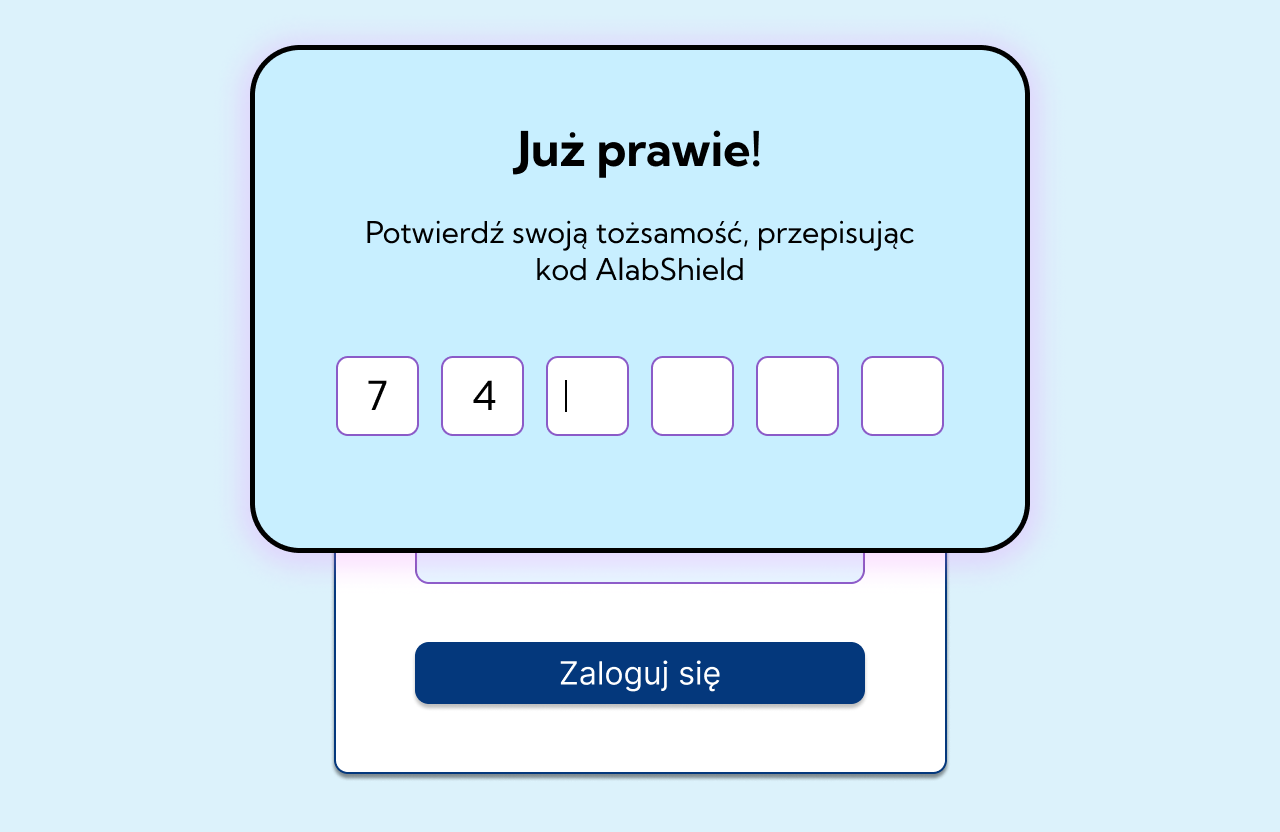
\includegraphics[width=0.8\textwidth]{2FA on log.png}
    \caption{Widok weryfikacji dwu stopniowej\label{fig:2FA}}
\end{figure}

\section{Dostęp do badań}

Badania są dostępne poprzez aplikację mobilną oraz stronę internetową w postaci wirtualnej.
Można też na podstawie badań wygenerować i pobrać z systemu pdf.
Wyniki badań są dostępne tylko dla uprawnionych osób.
Widok pobierania wyników jest przedstawiony na schemacie \ref{fig:results}.

\begin{figure}[h]
    \centering
    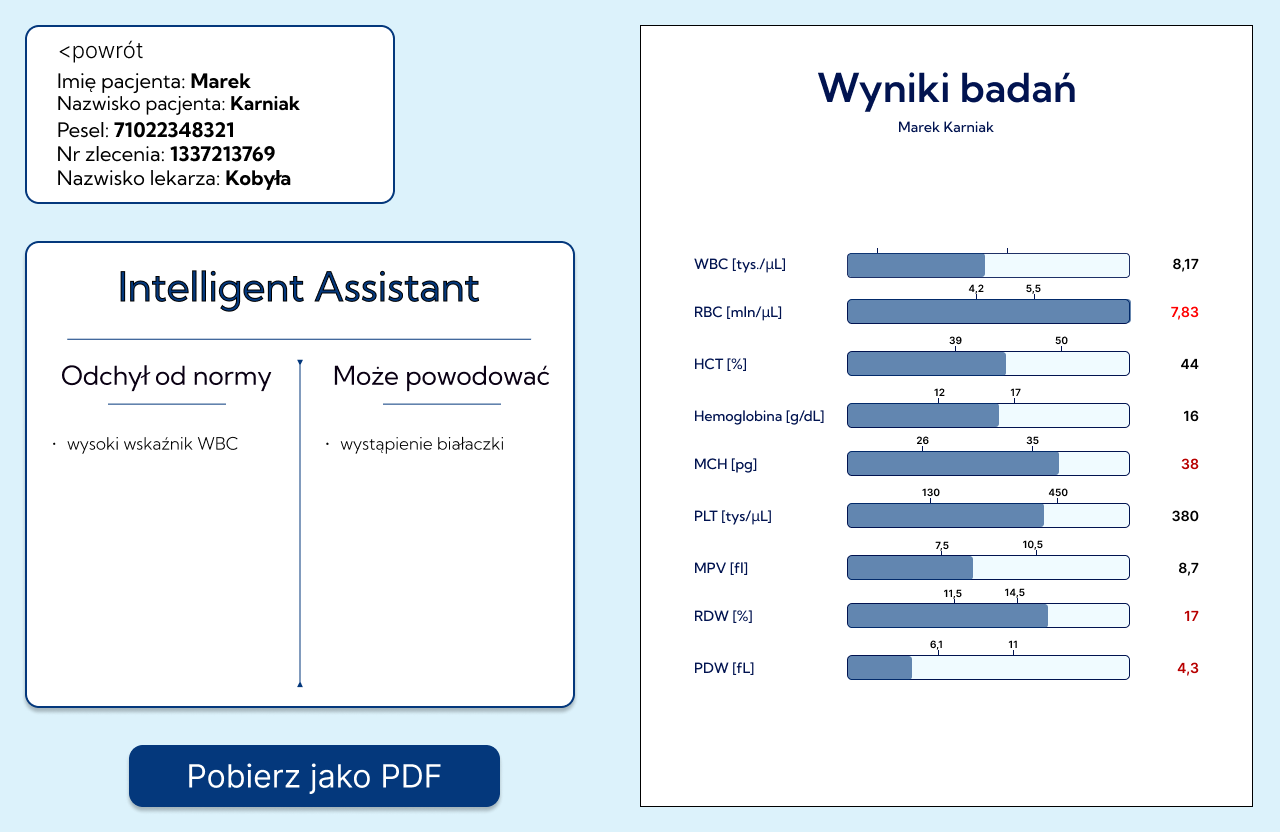
\includegraphics[width=0.8\textwidth]{wyniki-szpital.png}
    \caption{Widok pobierania wyników\label{fig:results}}
\end{figure}

\end{document}
